\subsection{Related Work}
\label{sec:relatedwork}

This section looks at projects we consider state-of-the-art in the context of
the Internet of Value. For each platform, we point out the limits that make it
unsuitable for the research problem, and we use these limits to back the gap
claims behind the research questions in Chapter~\ref{sec:aims}.

This section examines cutting-edge projects at the intersection of artificial intelligence
and blockchain technology, representing the evolving paradigm of the Internet of
Value. We analyze three pioneering platforms implementing AI agents on blockchain
networks: Virtuals Protocol, Autonolas, and Griffain. Each project demonstrates unique
approaches to autonomous on-chain entities, offering valuable insights into
architectural designs, governance models, and economic mechanisms. By understanding
their strengths and limitations, we can identify principles for developing next-generation
systems that maximize value creation while addressing current challenges. Before
diving into the specific projects, why do we need AI agents on the blockchain? The
answer lies in the need for autonomous systems that can operate with minimal human
intervention, enabling complex interactions with digital assets and smart
contracts. These agents can automate tasks, manage resources, and execute transactions
based on predefined rules or learned behaviors, thus enhancing the efficiency
and scalability of blockchain ecosystems. These systems typically employ a hybrid
architecture: AI decision-making occurs off-chain while execution happens on-chain
through transactions. This architectural paradigm has manifested in two primary approaches:

\begin{enumerate}
	\item \textbf{On-Chain AI Agents}: Entities represented on the blockchain as smart
		contract accounts or NFTs with associated wallets. These agents have an on-chain
		identity and can own assets directly, execute transactions, and participate
		in protocols autonomously. They might be governed through tokenization or DAOs \cite{Hassan2021}.

	\item \textbf{Off-Chain AI Agents with Transaction Authority}: Off-chain AI systems
		that have delegated authority to sign blockchain transactions. Recent
		account abstraction developments \cite{EIP7702, Buterin2021, Duan2024} enable users to safely
		delegate limited transaction powers to AI systems without exposing private
		keys.
\end{enumerate}

The projects analyzed below implement variations of these models, each with distinct
technical approaches and target use cases.

\subsubsection{Virtuals Protocol (Base L2, Ethereum)}

Virtuals Protocol enables the creation, co-ownership, and interaction with
tokenized AI agents, allowing shared economic ownership of autonomous digital entities
\cite{VirtualsWhitepaper2024}.

Each AI agent in Virtuals exists as an NFT with a token-bound smart contract account
implemented via ERC-6551 standard \cite{Wang2023}. This architecture gives each Agent
a persistent on-chain identity with its own wallet capabilities—the NFT itself can
hold assets and serve as a message sender for transactions. The AI logic (typically
a large language model) operates off-chain. Still, it can trigger on-chain
actions through the NFT's associated account.

The novelty of Virtuals lies in a novel shared ownership model. Each Agent is launched
with its own governance token\footnote{1 billion ERC-20 tokens minted per Agent},
creating a community of token holders who collectively govern and fund the Agent's
development \cite{VirtualsWhitepaper2024}. This tokenization enables fractional
investment in an agent's potential success—effectively turning AI agents into
community-owned assets. Governance token holders can participate in decision-making
about the Agent's capabilities, parameters, and resource allocation.

On the other hand, every Agent has to communicate with the GAME server via the
API key. Therefore, every reasoning runs on the proprietary server that can
return the response. Moreover, the disruption of the server agent is not able to
function correctly.

% \begin{figure}[!h]
% 	\centering
% 	% If you have a relevant image for Virtuals, add it here
% 	% \includegraphics[width=\columnwidth]{images/virtuals.png}
% 	\caption{Conceptual illustration of a token-bound AI agent on Virtuals
% 	Protocol}
% 	\label{fig:virtuals}
% \end{figure}

\subsubsection{Autonolas / Olas Network (Ethereum \& Multichain)}

Autonolas (OLAS) is a decentralized infrastructure for open-source autonomous
services and agents that began development in 2021, making it one of the first movers
in on-chain AI agents. It focuses on enabling "autonomous services that run off-chain
but interact on-chain and off-chain without restrictions" \cite{AICoin2023}.

Unlike Virtuals' NFT-centric approach, Autonolas separates the off-chain agent code
from on-chain coordination contracts. It provides an on-chain "agent registry." and
"service registry," where developers can publish agent implementations and
services that utilize them \cite{AICoin2023}. These agents often operate in multi-agent
configurations where several independent instances work together for fault tolerance.

The system leverages account abstraction extensively: Autonolas agents typically
interact with Ethereum via smart contract wallets. Multi-operator agent services might use threshold signatures
or multisig wallets to jointly manage on-chain actions, reducing single points
of failure. The platform operates across multiple EVM chains, including Ethereum
mainnet and several L2 networks \cite{OlasNetwork2024}.


The OLAS token provides governance rights and economic incentives within the ecosystem.
The platform implements crypto-economic mechanisms like staking and bonding
curves to reward both operators (who run agent instances) and developers (who build
agent code) \cite{OlasNetwork2024}. Revenue generated by agent services flows into
on-chain treasuries (typically Gnosis Safe contracts \cite{Liochon2023}) controlled by the service,
which then automatically distributes payouts to stakeholders.

% \begin{figure}[!h]
% 	\centering
% 	% If you have a relevant image for Autonolas, add it here
% 	% 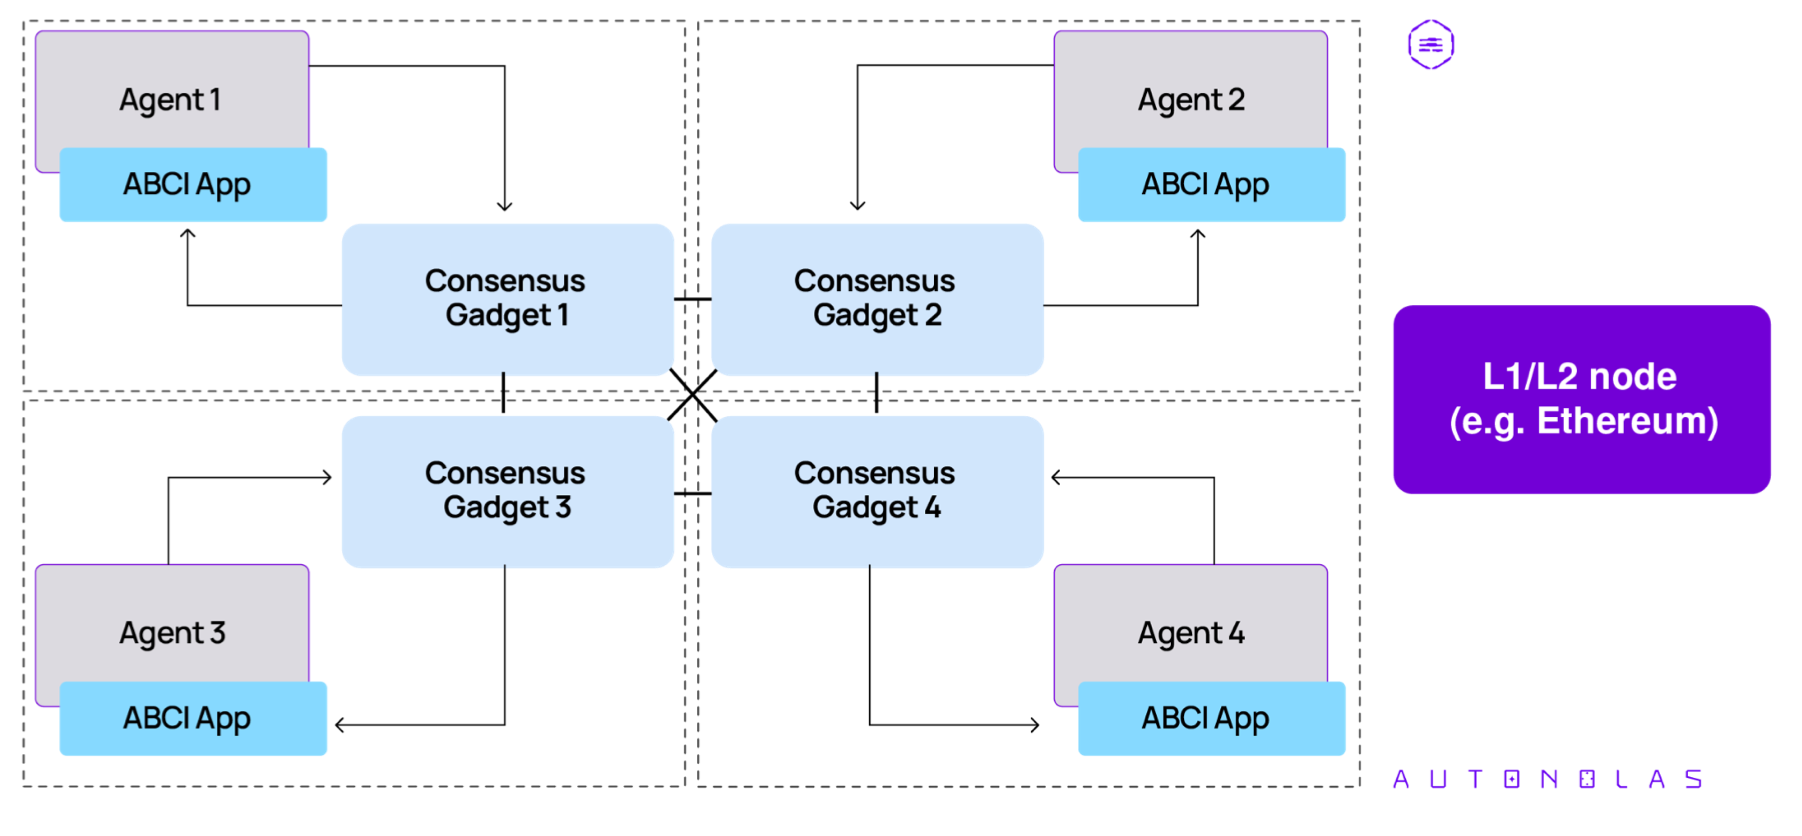
\includegraphics[width=\columnwidth]{images/autonolas.png}
% 	\caption{Multi-agent service architecture in Autonolas}
% 	\label{fig:autonolas}
% \end{figure}

\subsubsection{Griffain (Solana)}

Griffain is a rapidly growing platform for personal AI agents on the Solana
blockchain. The project's main goal is to simplify users' operations into
natural language without requiring a specialized user interface.

Griffain implements a seven-step model:
\begin{itemize}
	\item Action – User types "Swap 5 SOL to USDC".

	\item LLM parse – Runtime picks the swap action and parameters.

	\item Wallet check – Privy session signer verifies SOL balance.

	\item Route selection – Jupiter API returns the best path; Raydium pool if
		needed.

	\item Transaction builds \& sign – Execution service assembles SPL TokenSwap IX,
		signs with delegated key.

	\item Submit – Tx sent via Solana RPC; signature pushed to thread history.

	\item Billing – 1 Energy debited; user rewarded 0.25 Energy cashback.
\end{itemize}

When a user issues a command via the interface, natural language processing interprets
the intent and assigns the task to the relevant specialized Agent. For
transaction execution, Griffain employs a delegated wallet infrastructure (via
Privy), where each Agent operates through a Solana keypair linked to the user's
main wallet \cite{Griffain2024}. This design isolates agent activity—the Agent can
only access funds explicitly transferred to its delegated wallet. After we
approve the following command, the Agent picks up the best route using Jupiter API.
Upon returning instructions from the Jupiter API, a transaction is signed and submitted
to the Solana blockchain. Each action consumes energy, translating roughly 100 messages
(input-output from the LLM).

Unlike Virtuals' shared ownership model or Autonolas' protocol governance,
Griffain adopts a more traditional user-owns-agent approach. Each Agent belongs exclusively
to its creator, without fractional ownership or community governance. The GRIFFAIN
token serves primarily as a utility and speculative asset rather than a governance
mechanism for individual agents.

One disadvantage of the Griffain protocol is that agents may "hallucinate" irreversible
transfers. Despite safeguards, AI agents can still make wrong decisions. For
example, a trading agent might misinterpret a command and execute a bad trade.
Therefore, autonomy is limited for complex tasks. However, we can set up cron to
execute commands regularly.

\begin{table}[!htb]
	\centering
	\caption{Comprehensive Comparison of Blockchain AI Agent Platforms}
	\label{tab:ai-agents-detailed} \scriptsize
	\begin{tabular}{|p{1.8cm}|p{3.8cm}|p{3.8cm}|p{3.8cm}|}
		\hline
		\textbf{Parameter}            & \textbf{Virtuals Protocol}                      & \textbf{Autonolas}                               & \textbf{Griffain}                           \\
		\hline
		Blockchain                    & Base (Ethereum L2)                              & Ethereum + Multiple L2s                          & Solana                                      \\
		\hline
		Agent Identity                & ERC-6551 token-bound accounts (NFT with wallet) & Smart contracts with registry system             & Soulbound NFTs + delegated wallets          \\
		\hline
		AI Integration                & Off-chain LLMs with on-chain execution          & Multi-agent services with distributed operation  & Task-specific AI modules with NLP interface \\
		\hline
		Security Model                & Token governance for decision-making            & Multi-operator validation (threshold signatures) & Wallet delegation with spending limits      \\
		\hline
		Ownership Structure           & Fractional (community-owned via ERC-20)         & Protocol incentives for operators/developers     & Single-user ownership                       \\
		\hline
		Value Capture                 & Agent treasury + token appreciation             & Service fees distributed to stakeholders         & Platform token + service fees               \\
		\hline
		Monetization                  & Token markets with bonding curves               & Agent registry licensing fees                    & Platform token + transaction fees           \\
		\hline
		Primary Use Cases             & Entertainment, social agents, gaming            & DeFi automation, DAO governance, oracles         & Personal finance, trading automation        \\
		\hline
		Agent Autonomy                & Requires input from user                        & Agents can colaborate on multiple tasks           & Requires input from user                    \\
		\hline
		Modularity                    & Standardized IO ABI                             & plug-and-play services                             & forwarding input to other agent                    \\
		\hline
	\end{tabular}
\end{table} 

Our analysis of Virtuals Protocol, Autonolas, and Griffain reveals distinct approaches
to implementing AI agents on blockchain networks, each with unique strengths and
trade-offs. Table \ref{tab:ai-agents-detailed} provides a comprehensive comparison
across technical, economic, usage, and market dimensions.

\textbf{Virtuals Protocol} pioneered a community ownership model where AI agents
exist as tokenized entities (via ERC-6551) with their own on-chain treasuries.
This approach excels in creating economically aligned communities around AI
development but faces challenges in governance complexity and regulatory
uncertainty regarding tokenized AI assets.

\textbf{Autonolas} provides the most developed fault-tolerance model among the
surveyed systems, with a multi-agent architecture and cross-chain coordination
suited to mission-critical workloads. It does not, however, offer an account-level
primitive for agent delegation. Agents act through standard service contracts
rather than through accounts that carry their own policy, which leaves the
delegation gap identified in Chapter~\ref{sec:analysis} open.

\textbf{Griffain} prioritises user experience through a natural-language interface
on Solana. The trade-off is that decision-making is centralised in the platform
operator, and value assessment is reduced to direct execution with no support
for multi-dimensional evaluation or auditable human-in-the-loop voting. Griffain
therefore leaves the value-assessment and governance-support gaps unaddressed.

How are these platforms connected to the Internet of Value? That is an excellent
and valid question. Each of these platforms represents different visions for the
integration of AI and blockchain. Virtuals demonstrate how AI agents can become
community-owned digital assets with economic rights and governance structures. Autonolas
shows how decentralized, multi-agent systems can coordinate complex tasks with
enhanced security and reliability. Griffain illustrates how natural language interfaces
can make blockchain complexity accessible to mainstream users.

None of the surveyed platforms addresses all three gaps identified in this thesis:
multi-dimensional value assessment, agent-oriented on-chain primitives, and
auditable human-in-the-loop governance support. Virtuals leaves value assessment
to market dynamics, Autonolas does not provide an account-level primitive for
agent delegation, and Griffain trades autonomy for usability. Chapter~\ref{sec:design}
proposes an architecture designed to test whether these gaps can be closed
together rather than picked off one at a time.

Open challenges in balancing autonomy with safety, in regulatory treatment of
tokenised agents, and in keeping off-chain reasoning aligned with on-chain
execution remain across all three platforms. Chapter~\ref{sec:design} returns
to these challenges in the context of the gaps identified above.
